\section{Auswertung}
\label{sec:auswertung}

	Im Folgenden werden einige Mittelwerte, sowie deren Fehler berechnet.
	Dabei wird bei $n$ Messwerten $x_i$, der Fehler $\Delta x$ und der Mittelwert $x$ wie folgt berechnet:

	\begin{eqnarray*}
		x & = & \frac{1}{n}\sum_0^n{x_i} \,, \\
		\Delta x & = & \left(\frac{1}{n-1} \sum_0^n{(x - x_i)^2}\right)^\frac{1}{2} \,.
	\end{eqnarray*}

	\subsection{Brechungsindizes $n_\mathrm{i}$ in Abh"angigkeit der Wellenl"ange $\lambda$}
	\label{subsec:brechungsindizes}
		Zun"achst werden aus den Messdaten, die in Tabellen \ref{table:brechungsindizes} und \ref{table:eta} aufgef"uhrt sind, die Winkel $\varphi$ und $\eta$ bestimmt.
		Die Mittelung "uber die Daten aller Wellenl"angen $\lambda$ liefert mit Gleichung \eqref{eqn:phi}:

		\begin{equation*}
			\varphi = \SI{69.7 (11)}{\degree} \,.
		\end{equation*}

		Aus dem Versuchsaufbau geht jedoch hervor, dass alle Winkel des Prismas etwa $\varphi = \SI{60}{\degree}$ betragen m"ussen.
		Weil dieser Wert den tats"achlichen Aufbau des Prismas offensichtlich besser wiederspiegelt, wird dieser als Vergleichswert aufgef"uhrt.
		Die durch Rechnung mit $\varphi = \SI{60}{\degree}$ resultierenden Werte der Brechungsindizes $n_\mathrm{i}$ werden mit $n_\mathrm{opt}$ gekennzeichnet, die aus dem gemessenen Winkel $\varphi$ berechneten Werte mit $n$.
		Auf die Abweichung des gemessenen Wertes $n$ zum optimalen $n_\mathrm{opt}$ Wert wird in der Diskussion (\ref{sec:diskussion}) eingegangen.

		F"ur den Fehler $\Delta n$ der gemessenen Werte gilt nach Gau"sscher Fehlerfortpflanzung

		\begin{equation}
			\Delta n = \left|\frac{\sin\left(\frac{\eta}{2}\right)}{\cos(\varphi) - 1}\right| \Delta \varphi \,.
		\end{equation}

		Die Messwerte liefern anschlie"send mit Gleichung \eqref{eqn:brechungsindex} die in Tabelle \ref{table:brechungsindizes} aufgef"uhrten Brechungsindizes $n_\mathrm{opt}$ und $n$:

		\begin{table}[h!]
			\begin{center}
				\caption{Werte des Brechungsindex bei verschiedenen Wellenl"angen $\lambda$ \label{table:brechungsindizes}}
				\begin{tabular}{|c|c|c|c|c|c|c|}
					\hline
						Farbe & $\lambda [\SI{}{\nano \meter}]$ & $\varphi_\mathrm{l} [\SI{}{\degree}]$ & $\varphi_\mathrm{r} [\SI{}{\degree}]$ & $\varphi [\SI{}{\degree}]$ & $n_\mathrm{opt}$ & $n$ \\
					\hline 
					\hline
						gelb & $\SI{578.0}{}$ & $\SI{97.2}{}$ & $\SI{239.2}{}$ & $\SI{71.0}{}$ & $\SI{1.657}{}$ & $\SI{1.528(13)}{}$ \\
						gr"un & $\SI{546.1}{}$ & $\SI{97.8}{}$ & $\SI{239.0}{}$ & $\SI{70.6}{}$ & $\SI{1.652}{}$ & $\SI{1.524(13)}{}$ \\
						blaugr"un & $\SI{491.6}{}$ & $\SI{98.0}{}$ & $\SI{238.4}{}$ & $\SI{70.2}{}$ & $\SI{1.645}{}$ & $\SI{1.519(13)}{}$ \\
						violett & $\SI{404.7}{}$ & $\SI{99.0}{}$ & $\SI{237.6}{}$ & $\SI{69.3}{}$ & $\SI{1.634}{}$ & $\SI{1.511(13)}{}$ \\
						ultraviolett & $\SI{365.0}{}$ & $\SI{99.4}{}$ & $\SI{236.4}{}$ & $\SI{68.5}{}$ & $\SI{1.627}{}$ & $\SI{1.505(12)}{}$ \\
						ultraviolett & $\SI{366.3}{}$ & $\SI{99.6}{}$ & $\SI{236.2}{}$ & $\SI{68.3}{}$ & $\SI{1.625}{}$ & $\SI{1.504(12)}{}$ \\
					\hline 
				\end{tabular}
			\end{center}
		\end{table}

		% \begin{table}[h!]
		% 	\begin{center}
		% 		\caption{Messwerte zur Bestimmung von $\varphi$ \label{table:phi}}
		% 		\begin{tabular}{|c|c|c|c|c|}
		% 			\hline
		% 				Farbe & $\lambda [\SI{}{\nano \meter}]$ & $\varphi_\mathrm{l} [\SI{}{\degree}]$ & $\varphi_\mathrm{r} [\SI{}{\degree}]$ & $\varphi [\SI{}{\degree}]$ \\
		% 			\hline 
		% 			\hline
		% 				gelb         & $\SI{578.0}{}$ & $\SI{97.2}{}$ & $\SI{239.2}{}$ & $\SI{71.0}{}$\\
gr"un        & $\SI{546.1}{}$ & $\SI{97.8}{}$ & $\SI{239.0}{}$ & $\SI{70.6}{}$\\
blaugr"un    & $\SI{591.6}{}$ & $\SI{98.0}{}$ & $\SI{238.4}{}$ & $\SI{70.2}{}$\\
violett      & $\SI{404.7}{}$ & $\SI{99.0}{}$ & $\SI{237.6}{}$ & $\SI{69.3}{}$\\
ultraviolett & $\SI{365.0}{}$ & $\SI{99.4}{}$ & $\SI{236.4}{}$ & $\SI{68.5}{}$\\
ultraviolett & $\SI{366.3}{}$ & $\SI{99.6}{}$ & $\SI{236.2}{}$ & $\SI{68.3}{}$\\
		% 			\hline 
		% 		\end{tabular}
		% 	\end{center}
		% \end{table}		

		\begin{table}[h!]
			\begin{center}
				\caption{Messwerte zur Bestimmung von $\eta$ \label{table:eta}}
				\begin{tabular}{|c|c|c|c|c|}
					\hline
						Farbe & $\lambda [\SI{}{\nano \meter}]$ & $\Omega_\mathrm{l} [\SI{}{\degree}]$ & $\Omega_\mathrm{r} [\SI{}{\degree}]$ & $\eta [\SI{}{\degree}]$ \\
					\hline 
					\hline
						gelb         & $\SI{578.0}{}$ & $\SI{53.4}{}$ & $\SI{285.3}{}$ & $\SI{51.9}{}$ \\
gr"un        & $\SI{546.1}{}$ & $\SI{53.6}{}$ & $\SI{285.0}{}$ & $\SI{51.4}{}$ \\
blaugr"un    & $\SI{491.6}{}$ & $\SI{54.0}{}$ & $\SI{284.7}{}$ & $\SI{50.7}{}$ \\
violett      & $\SI{404.7}{}$ & $\SI{54.5}{}$ & $\SI{284.1}{}$ & $\SI{49.6}{}$ \\
ultraviolett & $\SI{365.0}{}$ & $\SI{54.9}{}$ & $\SI{283.8}{}$ & $\SI{48.9}{}$ \\
ultraviolett & $\SI{366.3}{}$ & $\SI{55.0}{}$ & $\SI{283.7}{}$ & $\SI{48.7}{}$ \\
					\hline 
				\end{tabular}
			\end{center}
		\end{table}		



	\subsection{Bestimmung der Dispersionsgleichung und deren Parameter $A_\mathrm{i}$}
	\label{subsec:dispersionskurve}
		Es werden zwei lineare Ausleichsrechungen der $\lambda^2$- $n^2$-, bzw. der $1 / \lambda^2$- $n^2$- Wertepaare f"ur Dispersiosngleichungen \eqref{eqn:dispersion1} und \eqref{eqn:dispersion2} durchgef"uhrt.
		Die Ausgleichsrechnung liefert die Koeffizienten $A_\mathrm{i}$ und $A'_\mathrm{i}$, sowie deren Fehler $\Delta A$.
		Dabei werden Koeffizienten bis $i = 2$ betrachtet.

		Daraus lassen sich die Abweichungsquadrate bei einer Anzahl von $z$ Messwerten wie folgt berechnen:

		\begin{eqnarray*}
			s^2 & = & \frac{1}{z - 2} \sum_{\mathrm{i} = 1}^z{\left(n^2(\lambda_\mathrm{i}) - A_0 - \frac{A_2}{\lambda_\mathrm{i}^2}\right)^2} \,, \\
			s'^2 & = & \frac{1}{z - 2} \sum_{\mathrm{i} = 1}^z{\left(n^2(\lambda_\mathrm{i}) - A'_0 + A'_2 \cdot \lambda_\mathrm{i}^2 \right)^2} \,. \\
		\end{eqnarray*}

		Die Ausgleichsrechnung liefert die Koeffizienten

		\begin{eqnarray*}
			A_0 & = & \SI{2.372(9)}{} \,, \\
			A_2 & = & \SI{1.509(103)e-14}{\meter \squared} \,, \\
			A_0' & = & \SI{2.217(6)}{} \,, \\
			A_2' & = & \SI{3.480(384)e11}{\per \meter \tothe{2}}\,. \\
		\end{eqnarray*}

		% Bei den gestrichenen Koeffizienten ist zu bemerken, dass der Fehler die Gr"o"senbegrenzng des Rechnerspeichers f"ur Flie"skommazahlen erreicht hat und daher einen unendlichen Wert liefert.
		% Dieser Wert hat keine physikalische Bedeutung, deutet aber schon darauf hin, dass die entsprechende Dispersionsgleichung nicht in der Lage ist, den vorliegenden Aufbau zu beschreiben.
		% Das wird deutlicher, wenn man die Abweichungsquadrate berechnet:

		Um eine Entscheidung f"ur eine der Dispersionsgleichungen zu treffen, werden die Abweichungsquadrate berechnet:

		\begin{eqnarray*}
			s^2 & = & \SI{0.03607}{} \,, \\
			s'^2 & = & \SI{0.03609}{} \,. \\
		\end{eqnarray*}

		Weil die Abweichung $s'^2$ f"ur Gleichung \eqref{eqn:dispersion2} gr"o"ser, als $s^2$ ist, wird die hier auftretende Dispersion durch Gleichung \eqref{eqn:dispersion1} beschrieben.
		Die folgenden Abbildungen \ref{fig:dispersion1} bis \ref{fig:dispersionNichtLinear} zeigen die Messwerte, sowie den Verlauf der Dispersionsgleichung.
		Die gew"ahlte Dispersionsgleichung \eqref{eqn:dispersion1} ist zudem in Abbildung \ref{fig:dispersionNichtLinear} nichtlinearisiert aufgetragen.

		\begin{figure}[h]
			\centering
			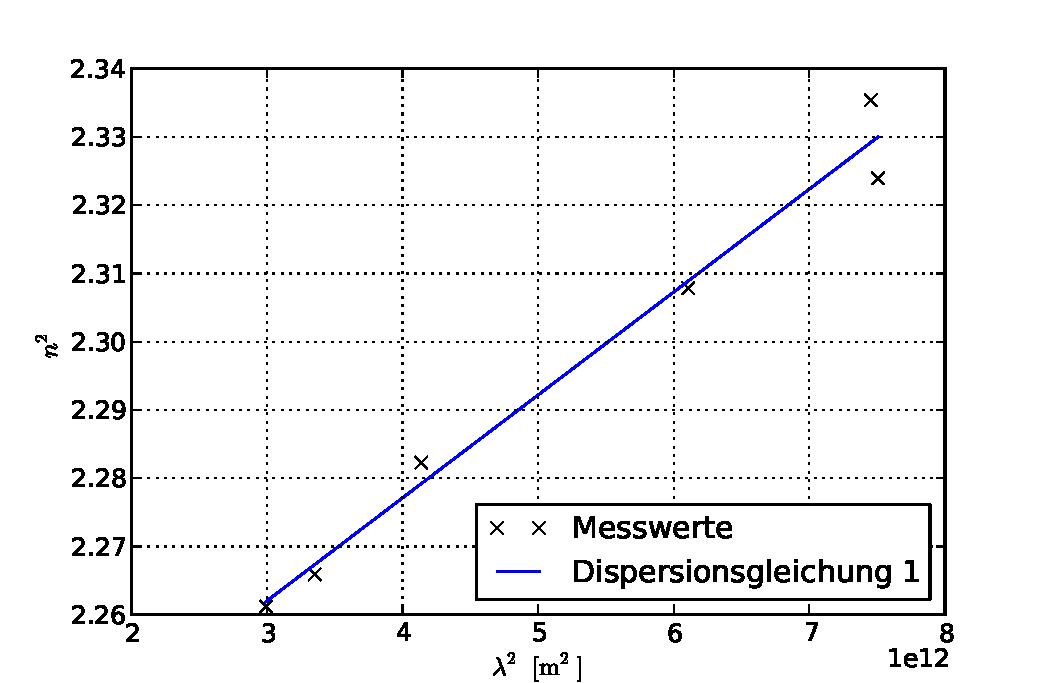
\includegraphics[width = 15cm]{img/dispersion1.pdf}
			\caption{Ausgleichskurve mit Hilfe von Gleichung \eqref{eqn:dispersion1} \label{fig:dispersion1}}
		\end{figure}

		\begin{figure}[h]
			\centering
			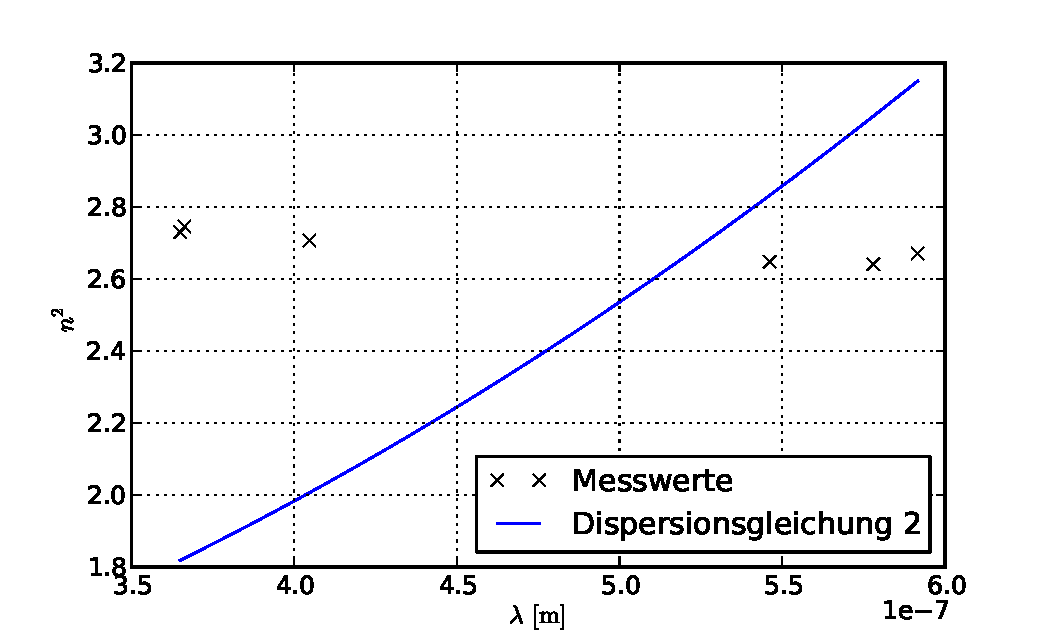
\includegraphics[width = 13cm]{img/dispersion2.pdf}
			\caption{Ausgleichskurve mit Hilfe von Gleichung \eqref{eqn:dispersion2} \label{fig:dispersion2}}
		\end{figure}

		\begin{figure}[h]
			\centering
			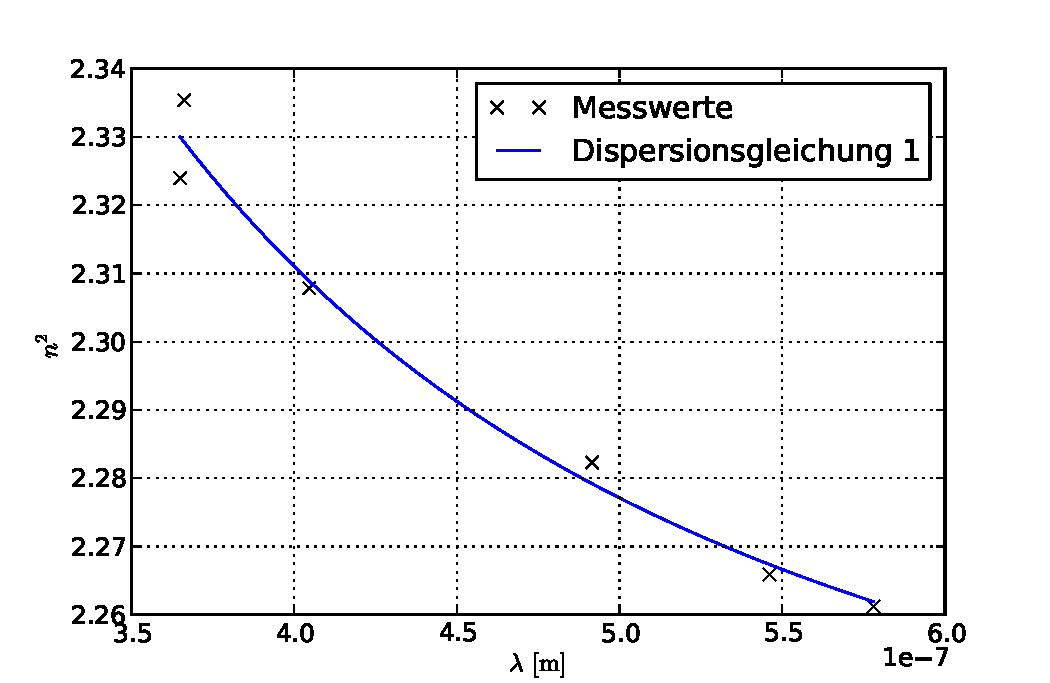
\includegraphics[width = 13cm]{img/dispersionNichtLinear.pdf}
			\caption{Theoriekurve der hier gew"ahlten Dispersionsgleichung \label{fig:dispersionNichtLinear}}
		\end{figure}

	\clearpage

	\subsection{Berechnung der Abbeschen Zahl $\nu$}
	\label{subsec:abbe}
		Mit Gleichung \eqref{eqn:abbe} und Kenntnis der Koeffizienten $A_0$ bis $A_2$ aus Kapitel \ref{subsec:dispersionskurve} l"asst sich die Abbesche Zahl bestimmen.
		Zun"achst werden die Brechungsindizes der Fraunhoferschen Linien bestimmt. Der dabei auftretende Fehler lautet

		\begin{equation*}
			\Delta n = \frac{1}{2}\left[\frac{1}{A_0 + \frac{A_2}{\lambda^2}}\left(\Delta {A_0}^2 + \frac{\Delta {A_2}^2}{\lambda^4}\right)\right]^\frac{1}{2}\,.
		\end{equation*}

		Die Dispersionsgleichung liefert zun"achst

		\begin{eqnarray*}
			n_\mathrm{C} & = & \SI{1.50061(208)}{} \,, \\
			n_\mathrm{D} & = & \SI{1.50341(216)}{} \,, \\
			n_\mathrm{F} & = & \SI{1.51018(240)}{} \,. \\
		\end{eqnarray*}

		Der Fehler der Abbeschen Zahl lautet

		\begin{equation*}
			\Delta \nu = \left[\left(\frac{1}{n_\mathrm{F}-n_\mathrm{C}}\right)^2 \Delta n_\mathrm{D}^2 + \left(\frac{n_\mathrm{D}-1}{(n_\mathrm{F}-n_\mathrm{C})^2}\right)^2\left(\Delta n_\mathrm{F}^2 + \Delta n_\mathrm{C}^2\right) \right]^\frac{1}{2}
		\end{equation*}

		Es wurde jeweils mit 11 Nachkommastellen gerechnet und es folgt

		\begin{equation*}
			\nu = \SI{52.60(1746)}{} \,.
		\end{equation*}

	\subsection{Das Aufl"osungsverm"ogen $A$ des Prismas}
	\label{subsec:aufloesungsvermoegen}
		Wie in Kapitel \ref{sec:durchfuehrung} gezeigt, gilt mit einer Basisbreite $b$ des Prismas f"ur das Aufl"osungsverm"ogen:

		\begin{equation*}
			A = \frac{\lambda}{\Delta \lambda} = b \frac{\partial n}{\partial \lambda} \,.
		\end{equation*}

		Mit der hier genutzten Dispersionsgleichung \eqref{eqn:dispersion1} gilt f"ur das Aufl"osungsverm"ogen $A$ und den entsprechenden Fehler $\Delta A$:

		\begin{eqnarray*}
			A & = & b \frac{A_2}{\lambda^3} \frac{1}{\sqrt{A_0 + \frac{A_2}{\lambda^2}}} \,, \\
			\Delta A & = & \left[\left(\frac{b A_2}{2 \lambda^3 \left( A_0 + \frac{A_2}{\lambda^2} \right)^\frac{3}{2}} \right)^2 \Delta A_0^2 + 
				\left[\frac{b}{\lambda^3 \left(A_0 + \frac{A_2}{\lambda^2}\right)^\frac{1}{2}} - \frac{A_2 b}{2\lambda^5 \left(A_0 + \frac{A_2}{\lambda^2}\right)^\frac{3}{2}}\right]^2 \Delta A_2^2
			\right]^\frac{1}{2} \,.
		\end{eqnarray*}

		\clearpage

		Bei einer Basisl"ange $b = \SI{3}{\centi \meter}$ folgt f"ur das Aufl"osungsverm"ogen des hier vorliegenden Prismas bei den Fraunhoferwellenl"angen $\lambda_\mathrm{C} = \SI{656}{\nano \meter}$ und $\lambda_\mathrm{F} = \SI{486}{\nano \meter}$:

		\begin{eqnarray*}
			A_\mathrm{C} & = & \SI{1068(66)}{} \,, \\
			A_\mathrm{F} & = & \SI{2611(165)}{} \,. \\
		\end{eqnarray*}

	\subsection{Berechnung des n"achsten Absorptionspunktes $\lambda_\mathrm{1}$}
	\label{subsec:absorptionspunkt}
		Durch Koeffizientenvergleich in Formeln \eqref{eqn:dispersion1} und \eqref{eqn:dispersion1exakt} erh"alt man

		\begin{eqnarray*}
			A_0 & = & 1 + \frac{N_1 q_1^2 \lambda_1^2}{4 \pi^2 c^2 \epsilon_0 m_1} \,, \\
			A_2 & = & \lambda_1^2 (A_0 - 1) \,, \\
			\Rightarrow \quad \lambda_1 & = & \sqrt{\frac{A_2}{A_0 - 1}} \,, \\
			\Delta \lambda_1 & = & \left[\frac{1}{4}\frac{A_2}{(A_0 - 1)^3} \Delta {A_0}^2 + \frac{1}{4}\frac{1}{A_2 (A_0 - 1)} \Delta {A_2}^2\right]^\frac{1}{2} \,.
		\end{eqnarray*}

		Mit den Koeffizienten $A_0$ und $A_2$ aus Kapitel \ref{subsec:dispersionskurve} l"asst sich also der Wert $\lambda_1$ der n"achsten Absorptionsstelle finden:

		\begin{equation*}
			\lambda_1 = \SI{111.3(38)}{\nano \meter} \,.
		\end{equation*}
